\begin{frame}
  \frametitle{Barnes-Hut}
 \begin{columns}[T] % align columns
 \begin{column}{.48\textwidth}
  \begin{itemize}
      \item Clustering
      \item Typical subdivision
      \begin{itemize}
          \item Quad and octree
          \item Width of region
      \end{itemize}
      \item Threshold
  \end{itemize}
\end{column}
 \begin{column}{.48\textwidth}
  \begin{figure}
      \centering
      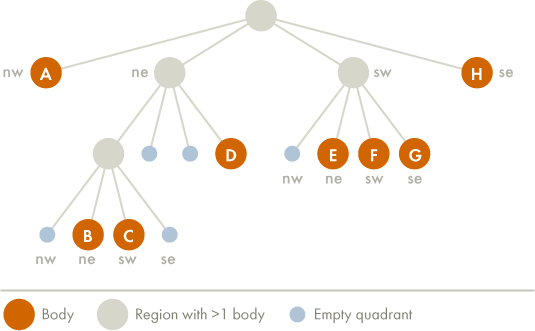
\includegraphics[width=0.8\textwidth]{../report/assests/example-tree.png}
      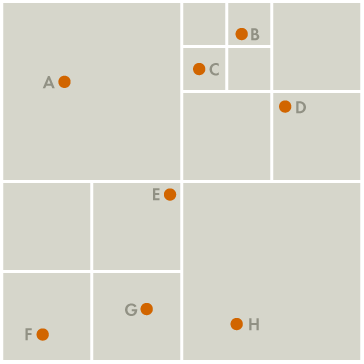
\includegraphics[width=0.47\textwidth]{../report/assests/example-space.png}
      \caption{A quadtree and the equivalent space it is constructed from.}
      \label{fig:subdivision}
  \end{figure}
  \end{column}
  \end{columns}
\end{frame}

\begin{frame}{Radix-tree}
   \begin{columns}[T]
   \begin{column}{.48\textwidth}
      \begin{itemize}
          \item Mapping locality
          \item Morton code
          \item Parallel construction
          \begin{itemize}
              \item One thread per internal node.
              \item Prefix length
              \item Split position
          \end{itemize}
          \item Easy to generalize to $n$-dimensions
      \end{itemize}
   \end{column}
   \begin{column}{.48\textwidth}
   \begin{figure}
      \centering
      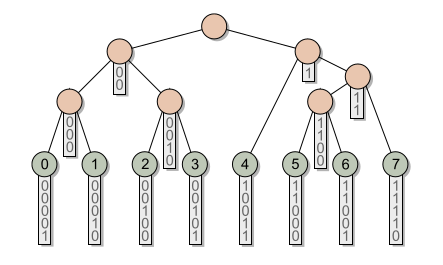
\includegraphics[width=0.8\textwidth]{../report/assests/radix.png}
      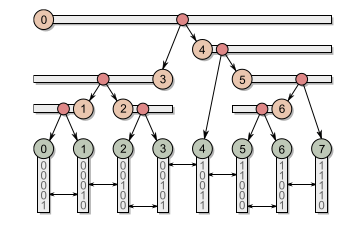
\includegraphics[width=0.8\textwidth]{../report/assests/radix-split.png}
      \caption{An example of a binary radix-tree}
      \label{fig:radix}
  \end{figure}
  \end{column}
  \end{columns}
\end{frame}{}
